\documentclass[12pt]{article}

\usepackage{amsmath, amsthm, amssymb, amsbsy, amsfonts}
\usepackage[plainpages=false,pdfpagelabels]{hyperref}
\hypersetup{
    colorlinks,
    citecolor=black,
    filecolor=black,
    linkcolor=black,
    urlcolor=blue
}
\usepackage{verbatim}
\usepackage{enumitem}
\usepackage[utf8x]{inputenc}

% Redefine the \vec command to use bold font instead of an arrow
\renewcommand\vec[1]{\mathbf{#1}}

%\def\nl{\hfill\break\null}
\oddsidemargin=0.3cm
\topmargin=-1cm
\textwidth=15cm
\textheight=23cm
\parindent=0cm
\parskip=1mm


\usepackage{graphicx}
\DeclareMathOperator*{\argmin}{argmin}

\newenvironment{enumialpha}{\begin{enumerate}
  \def\theenumi{\alph{enumi}}
  \def\labelenumi{(\theenumi)}}{\end{enumerate}}

\newenvironment{enumiiroman}{\begin{enumerate}
  \def\theenumii{\roman{enumii}}
  \def\labelenumii{(\theenumii)}}{\end{enumerate}}


\begin{document}

\begin{tabular*}{15cm}{@{}l@{\extracolsep{\fill}}r}
  Albert-Ludwigs-Universit\"at Freiburg, Institut f\"ur Informatik \\
PD Dr. Cyrill Stachniss \\  Lecture: Robot Mapping \\
  Winter term 2013 
\end{tabular*}

\bigskip


\begin{center}
{\bf \Large Sheet 9}

{\large Topic: Least-Squares}

Submission deadline: January, 27\\
Submit to: \texttt{robotmappingtutors@informatik.uni-freiburg.de}
\end{center}

\subsubsection*{Exercise: Odometry Calibration}

Implement an odometry calibration tool based on a least-squares method
as presented in the lecture. To support this task, we provide a small
\emph{Octave} framework (see course website).  The framework contains
the following folders:

\begin{description}
\item [data]
  contains the recorded raw odometry and the motion estimated by a
  scan-matcher for each time step.
\item [octave]
  contains the Octave framework with stubs to complete.
\item [plots]
  this folder is used to store images.
\end{description}

The below mentioned tasks should be implemented inside the framework in
the directory \texttt{octave} by completing the stubs:
\begin{itemize}
  \item
    Implement the functions in \texttt{ls\_calibrate\_odometry.m} for
    constructing and solving the least-squares system.
  \item
    Implement the function in \texttt{apply\_odometry\_correction.m} for
    applying the calibration matrix to a set of odometry measurements.
  \item
    Implement the function in \texttt{compute\_trajectory.m} for
    chaining up the affine transformation matrices of the relative
    odometry measurements.
\end{itemize}

\begin{figure}
  \centering
  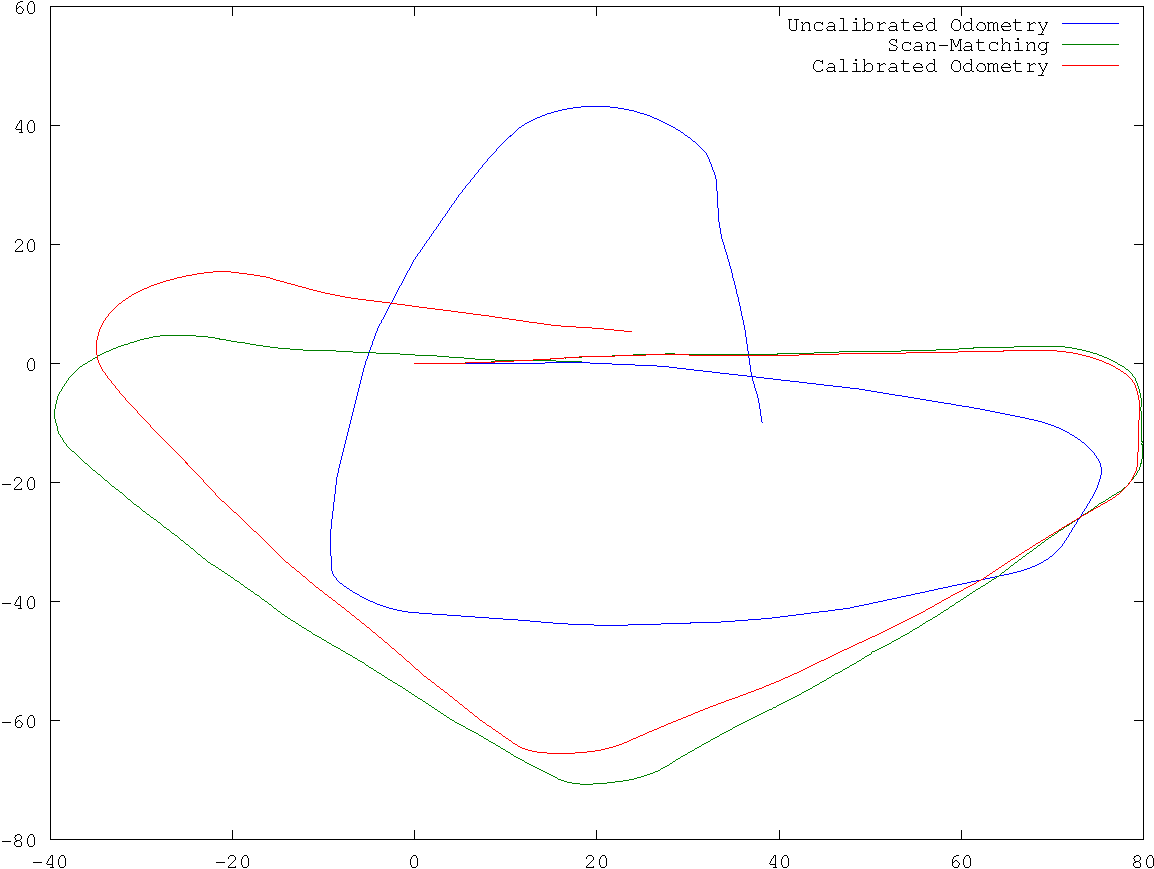
\includegraphics[width=0.8\columnwidth]{odometry-calibration}
  \caption{Visualization of the uncalibrated odometry, scan-matching,
  and the odometry after calibration.}
  \label{fig:result}
\end{figure}

After implementing the missing parts, you can run the framework.  To do
that, change into the directory octave and launch \emph{Octave}. To
start the main loop, type \texttt{LSCalibrateOdometry}.  The script will
produce a plot showing the trajectory of the raw odometry measurements,
the estimate obtained by scan-matching, and the odometry after applying
the calibration.  This plot will be saved in the \texttt{plots}
directory. Figure~\ref{fig:result} shows the result that you should obtain.

\newpage
Some implementation tips:
\begin{itemize}
  \item
    The functions \texttt{v2t} and \texttt{t2v} are available within the
    framework and allow to convert between a vector representing the
    pose of a robot and its corresponding affine transformation matrix.
  \item
    The function \texttt{reshape} returns a matrix with specified
    dimensions whose elements are taken from another matrix. It can, for
    example, convert a vector into a matrix.
  \item
    Many of the functions in \emph{Octave} can handle matrices and
    compute values along the rows or columns of a matrix. Some useful
    functions that support this are \texttt{sum},  \texttt{log},
    \texttt{sqrt}, \texttt{sin}, \texttt{cos}, and many others.
\end{itemize}

\end{document}
